\chapter{Introducció}
En aquest treball intentaré posar a prova la seguretat de les contrasenyes. Sovint, acostumem a guardar-nos la mateixa contrasenya per totes les aplicacions que utilitzem, sigui per facilitat o comoditat. Però aquesta facilitat que busquem havent de posar la mateixa contrasenya en totes les aplicacions/pàgines ens pot portar algun problema? Això és el que vull demostrar en aquest treball de recerca, que tan difícil és desxifrar una contrasenya bàsica que acostumem a guardar, i també comprovar la seguretat de les contrasenyes automàtiques que ens ofereixen moltes aplicacions amb l'etiqueta de 'contrasenya segura'.

\section{Context i motivació}
Avui en dia estem en una societat on guardem pràcticament totes les nostres dades a la xarxa. Aquestes van des de dades personals, fins a la nostra targeta de crèdit o la nostra ubicació.\\
Mitjançant les dades de l'estudi anual \textit{Password Decisions Survey} de l'empresa Bitwarden (2023), podem observar un gràfic sobre la reutilització de contrasenyes:

% --- INSERCIÓ DE LA IMATGE ---
\begin{figure}[h!]
    \centering
    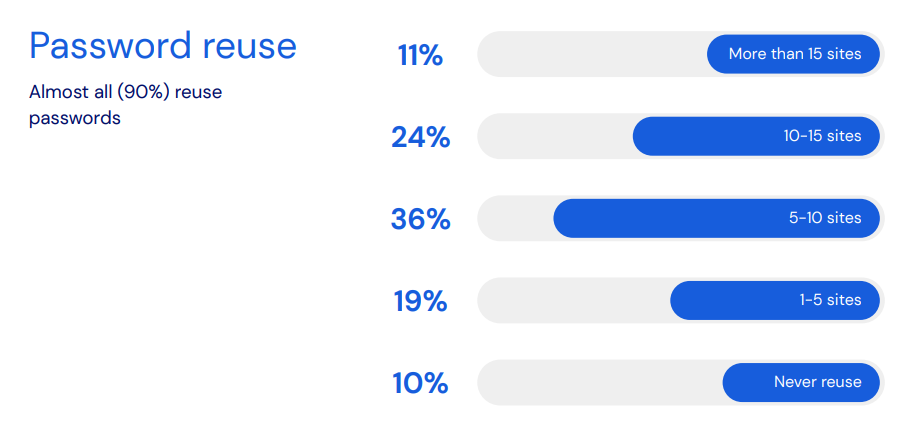
\includegraphics[width=0.85\textwidth]{bitwarden.png}
    \caption{Percentatge de llocs web on els usuaris reutilitzen la mateixa contrasenya. \textit{Font: Elaboració pròpia a partir de dades de Bitwarden (2023).}}
    \label{fig:reutilitzacio_contrasenyes}
\end{figure}
\begin{table}[h!]
    \centering
    \renewcommand{\arraystretch}{1.3} % Dona una mica d'aire a les files
    \begin{tabular}{|l|c|}
        \hline
        \textbf{Nombre de llocs web on es reutilitza} & \textbf{Percentatge d'usuaris} \\ \hline
        Més de 15 llocs web & 11\% \\ \hline
        Entre 10 i 15 llocs web & 24\% \\ \hline
        Entre 5 i 10 llocs web & 36\% \\ \hline
        Entre 1 i 5 llocs web & 19\% \\ \hline
        Mai les reutilitzen & 10\% \\ \hline
    \end{tabular}
    \caption{Desglossament de l'hàbit de reutilització de credencials.}
    \label{tab:dades_bitwarden}
\end{table}
\newpage 
% -----------------------------
\noindent Com es pot observar a la Figura \ref{fig:reutilitzacio_contrasenyes}, segons Bitwarden el 90\% dels usuaris reutilitza la seva contrasenya. El més abundant és la reutilització entre 5 i 10 pàgines web.
Aquest estudi ens demostra que per comoditat, la gent no s'esforça per canviar la contrasenya en les diferents webs. Això pot ser un perill, ja que a l'utilitzar la mateixa contrasenya en una web de baixa seguretat i en el teu compte del banc pot fer que la vulnerabilitat de seguretat d'un lloc poc important acabi obrint la porta a llocs on guardem informació més confidencial.\\

\noindent Com a usuari que tendeix a fer servir la mateixa contrasenya per tot, he desenvolupat un interès en l'ambit de la ciberseguretat, i sumant-li també el meu interès a la programació, m'han portat a escollir aquesta idea de treball de recerca.

\section{Objectius}
L'objectiu principal del treball de recerca és desenvolupar un programa capaç de mesurar i analitzar el temps necessari per desxifrar les contrasenyes que els usuaris solen utilitzar només perquè són 'fàcils de recordar', i comparar la seguretat d'aquestes contrasenyes amb les que algunes webs et proporcionen com a 'Contrasenya segura'.\\
Per assolir aquest objectiu general faré les següents tasques:
\begin{itemize}
    \item Desenvolupar un programa capaç de realitzar atacs de força bruta.
    \item Comparar el temps de desxifrat segons la longitud de la clau i els caràcters utilitzats
    \item Avaluar l'eficiència de les contrasenyes generades aleatòriament en comparació a les creades manualment.
\end{itemize}

\section{Hipòtesi}
Plantejo d'hipòtesi que una contrasenya generada automàticament serà molt més segura que la majoria de contrasenyes que elabori l'usuari, ja que acostumen a tenir més caràcters i combinar diferents tipografies, com les majúscules, els punts, els números. Fent-les així pràcticament impossible de desxifrar sumant-li que normalment tenen uns 12 caràcters.
